\documentclass[jou]{apa6}

\usepackage[american]{babel}

\usepackage{csquotes}
\usepackage[style=apa,sortcites=true,sorting=nyt,backend=biber]{biblatex}
\DeclareLanguageMapping{american}{american-apa}
\addbibresource{bibliography.bib}

\title{Advantages of Object-Based Audio and Possible Future Optimizations}

\author{Nianze Liu}
\affiliation{New York University}

\leftheader{Liu}

\abstract{This article firstly goes through the advantages of object-based audio compared with traditional channel based audio as well as sound field representation, leading to the discussion of possible optimizations to current object-based audio production workflow. In order to make the pipeline more productive, the concept of Internet of Things is introduced with some real world demonstration, ending with a brief discussion about the future challenges in combining Internet of Things into the field of immersive audio.}

\keywords{Immersive Audio, Internet of Things, Object-Based Audio}

\begin{document}
\maketitle

\section{Introduction}

With its flexibility to dynamically render the output audio according to the context requirement at runtime, object-based audio becomes more and more popular nowadays, especially in the field of virtual reality and augmented reality. 

\section{Advantages of Object-Based Audio}

Traditionally, in order to get best playback quality, producer dealing with channel-based audio must have the knowledge of the target reproduction system, as shown in Figure~\ref{fig:Figure1}: for headphone setup, binaural recordings will provide better experience; for loudspeakers, stereo microphones are preferred during the recording phase. In the end, for different reproduction devices setup, upmixing and downmixing, as well as signal processing accordingly, are required to optimize the playback experience, which is inflexible, if not unrealistic, in the context of immersive audio since we might want the audio to be dynamically updated according to the listener's head direction. Object-based audio, as showed in \textcite{susal2016immersive}, has the advantage of being format-agnostic, which makes it more efficient to produce high quality audio playback.

\begin{figure}[h!]
    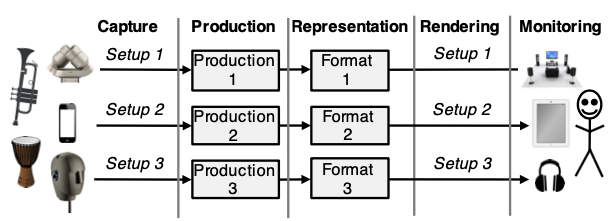
\includegraphics[width=\linewidth]{channel_based.png}
    \caption{Channel Based Pipeline}
    \label{fig:Figure1}
\end{figure}

There is another audio representation that could be used in immersive audio: sound field representation. However, sound field representation has a big disadvantage: the PCM channels required to encode more detailed spacial information grows very quickly: in Higher-Order Ambisonics, 1st order requires 4 channels, 2nd order requires 9 channels, and 3rd order grows up to 16 channels. For practical reasons, soud field representation might be more appropriate with lower order in the context of 3 degrees of freedom (DOF) playback scenarios. For more immersive 6 DOF environment, object-based audio representation is preferred. What's more, with the associated audio metadata, it is easier to modify object-audio representation to provide better interactivity and achieve spacial fidelity compared to the sound field representation.

\section{Optimizing Object-Based Audio Workflow}

\subsection{Pipeline Optimization}

With all the advantages above, object-based audio is a promissing immersive audio representation. However, current workflows in object-based audio production have not reached its full potential.

First, in the capture phase, the object-based audio is usually created manually by producers. This could be optimized by adopting new recording facilities able to directly generate metadata and create object-based audio. For example, in \textcite{coleman2018audio}, a kinect2 sensor is used to get position data, which will be directly encoded into the audio object metadata.

Second, in the production phase, there are multiple different formats to represent the metadata, such as Audio Scene Discription Format(ASDF) and SpatDIF, where ASDF contains the complete scene information in a static file, inlucding the whole temporal progress, while SpatDIF has limited extensibility. According to \textcite{coleman2018audio}, it is suggested to adopt the more flexible JSON format, which is widely used in the internet as a versatile means to represent object-oriented information. The proposed JSON format is a streaming representation, so the temporal change of audio scene could be transmitted repeatedly via a network connection. An example hierarchy of this JSON representation is shown in Figure~\ref{fig:Figure2} below:

\begin{figure}[h!]
    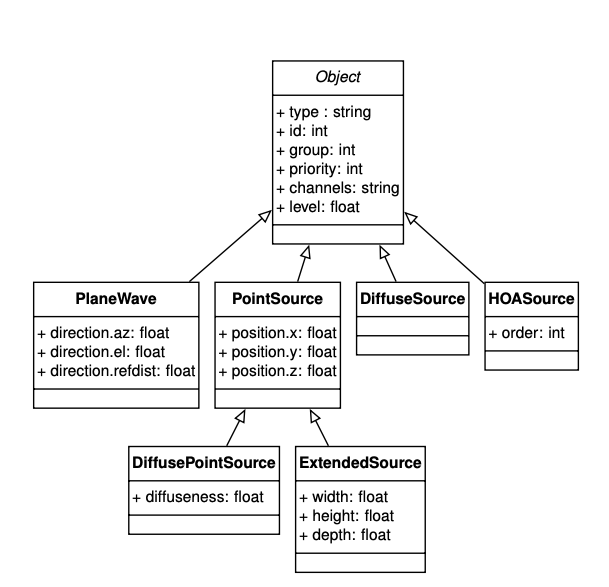
\includegraphics[width=\linewidth]{hierarchy.png}
    \caption{JSON type metadata hierarchy}
    \label{fig:Figure2}
\end{figure}

Last but not least, in the rendering phase, it is preferred to follow the component-based design pattern with predefined application programming interfaces(API) shared by the whole industry, so that software frameworks can be built in small modules, and extensibility and portability might be achieved more easily. Modules might focus on the signal pocessing part, as well as the signal's interaction part. With the common API, the modules could be easily updated, exchanged and switched, making the rendering procedule more flexible.

\subsection{Assisted with Internet of Things}

To make the object-based audio pipeline more productive, techniques from Internet of Things might be helpful. 

Internet of Things, according to \textcite{turchet2018internet}, refers to "embedded systems that are connected to the internet, which are able to interact with each other and cooperate to reach common goals." Following this direction, in \textcite{lee2017location}, speakers are combined with beacon and Raspberry Pi to form a group of smart speakers that are aware of their relative positions in respect to other speakers. If we go one step further, by embedding sensors in recording devices, it is also possible to build next generation of "smart microphones" that are smart enough to directly generate object-based audio metadata by communicating with each other smart devices.

Since the optimized object-based audio pipeline uses standardized JSON format for the audio object metadata as well as component-based common API, it is even possible for the capture devices to communicate with the devices in the later production phases. For example, it is possible to build smart instruments, which is able to send signals to digital audio workstation (DAW) about the instruments' state such as automatic transcription, synthesizer modes, and current sound effects. It is also possible to play the instrument in the virtual reality to make a more immersive networked music performance.

\section{Future Challenges}

It is exciting to apply Internet of Things to the field of immersive audio. However, there are still engineering challenges before their complete merge. If we want to connect everything in a network, the low-latency high quality audio streams over this network music be available. In the case of networked music performance, there's another synchronization issue for audio streams in different time zones. Another challenge comes from the standardization: if we want to build a network of everything, then smart devices need to communicate with each other in the same language. How to make such a standard that covers different people's needs requires more research and efforts.

\printbibliography

\end{document}